%% Copyright 2007, 2008, 2009 Elsevier Ltd

\documentclass[preprint,12pt]{elsarticle}

\usepackage{verbatim} % comentarios
\usepackage{epsfig}
\usepackage{amssymb} 

\usepackage{mathtools}

\usepackage{lineno}

\usepackage{tikz}        %permite rellenar las figuras (circulos)
\usepackage{etoolbox}
%\usepackage[backend=biber,citestyle=authoryear]{biblatex}
\usepackage{ulem}         %permite el tachado de texto.

%\usepackage{epstopdf}


\usepackage[caption=false]{subfig}

\begin{document}

\newcommand*{\hwplotB}{\raisebox{3pt}{\tikz{\draw[red,dashed,line 
width=3.2pt](0,0) -- 
(5mm,0);}}}

\newrobustcmd*{\mydiamond}[1]{\tikz{\filldraw[black,fill=#1] (0,0) -- 
(0.1cm,0.2cm) --
(0.2cm,0) -- (0.1cm,-0.2cm);}}

\newrobustcmd*{\mytriangleleft}[1]{\tikz{\filldraw[black,fill=#1] (0,0.15cm) -- 
(-0.3cm,0) -- (0,-0.15cm);}}
\definecolor{Blue}{cmyk}{1.,1.,0,0} 

\begin{frontmatter}


\title{Effects of the body force on the pedestrian and the evacuation dynamics}


\author[add1]{I.M.~Sticco}
 \address[add1]{Departamento de F\'\i sica, Facultad de Ciencias 
Exactas y Naturales, \\ Universidad de Buenos Aires,\\
 Pabell\'on I, Ciudad Universitaria, 1428 Buenos Aires, Argentina.}

 \author[add2]{G.A.~Frank}
 \address[add2]{Unidad de Investigaci\'on y Desarrollo de las 
Ingenier\'\i as, Universidad Tecnol\'ogica Nacional, Facultad Regional Buenos 
Aires, Av. Medrano 951, 1179 Buenos Aires, Argentina.}

\author[add1,add3]{C.O.~Dorso\corref{cor1}}%
 \cortext[cor1]{codorso@df.uba.ar}

 \address[add3]{Instituto de F\'\i sica de Buenos Aires,\\
Pabell\'on I, Ciudad Universitaria, 1428 Buenos Aires, Argentina.}
 



\begin{abstract}

The Social Force Model (SFM) is a suitable model for describing crowd behaviors
\textcolor{blue}{under emotional stress}.
This research analyzes the role of the body force in the original SFM.
We focused on the parameter associated with the body stiffness ($k_n$) and its impact on the pedestrian
dynamics for two different geometries: bottlenecks and corridors.
Increasing $k_n$ produces opposite effects on \textcolor{blue}{crowd dynamics for each geometry}: an increase of the crowd velocity 
for bottlenecks, and a decrease for corridors. 
The former reflects the fact that \textcolor{blue}{an increase in the stiffness reduces
the overlap between pedestrians and, as a consequence, the sliding friction is reduced.} 
This phenomenon reduces the number of blocking clusters close to the exit door. 
\textcolor{blue}{In the case of the corridor, instead, due to the confining walls,
the pedestrians get tight }
 into a lattice-like configuration due to space limitations.
The friction interaction with the walls determines the velocity of the whole crowd along the corridor.
Additionally, the corridor geometry \textcolor{blue}{generates} a flux slowing down for very
crowded environments, as observed in many real-life situations.
We also explored the dimensionless parameters that arose from the reduced-in-units
equation of motion and tuned them to reproduce the qualitative behavior of the empirical fundamental diagram. 

\end{abstract}

\begin{keyword}

Pedestrian Dynamics \sep Social Force Model \sep Body Force


\PACS 45.70.Vn \sep 89.65.Lm

\end{keyword}

\end{frontmatter}

%\linenumbers

\section{\label{introduction}Introduction}

The Social Force Model (SFM) models the crowd dynamics 
considering three kinds of force: desired forces, social forces, and physical forces.
In its original version, the SFM, addresses two physical forces as essential: 
 the ``body force'' and the ``sliding friction''. Both are 
inspired by granular interactions and were claimed to be necessary  
for attaining the particular effects in panicking crowds \cite{helbing_2000}. 
The ``sliding friction'' actually proved to be an essential feature of the 
``faster-is-slower'' effect, although the role of the ``body force'' appears, 
at a first instance, not so clear \cite{dorso_2005,dorso_2007,dorso_2011}. \\ 

The existence of a ``body force'' in the context of highly dense crowds (say, 5 
to 10$\,$people/m$^2$) is a commonsense matter \cite{henein_2007,fruin_1993}. 
Researchers, however, question the numerical setting for this force in 
the SFM context \cite{lakoba_2005}. As a matter of fact, the usual 
\textcolor{blue}{\sout{setting by} set of parameters provided by }
Helbing prevents the excessive overlapping among pedestrians, but it is known to 
accomplish artificially high force levels 
\cite{helbing_2000,lakoba_2005,langston_2006,lin_2017}. The force estimates 
from the SFM appear to be remarkably higher with respect to the reported real 
life data (say, an order of magnitude). The crowd motion simulations, however, 
present \textcolor{blue}{\sout{quite}} realistic results \cite{lakoba_2005,langston_2006,dorso_2017}. 
The 
point seems to be that the SFM focuses on the ``collective behavior'' due 
to clogging, missing the ``individualistic'' perspective  of single pedestrians 
or very small groups \cite{helbing_2000,henein_2007,narain_2009}.  \\ 

Many researchers realized that modifying the SFM may (partially)
\textcolor{blue}{\sout{ surpass the misleading parameter setting}
fix the misleading results}. It was proposed that the pedestrians' 
psychological force (say, the ``social force'') should be suppressed in the 
context of highly dense crowds 
\cite{pelechano_2007,moussaid_2011,alonso_2014,bottinelli_2017}, or smoothly 
quenched according to the crowd density \cite{song_2019}. The authors in 
Refs.~\cite{kabalan_2017,jebrane_2019} further proposed a rigid body model in 
order to completely avoid the overlapping phenomenon. This perspective 
dismisses 
any connection to a ``sliding friction''. Conversely, other authors tried to 
limit the pedestrians acceleration by introducing ``static friction'' between 
the pedestrians and the floor \cite{wang_2019}. This kind of friction, however, 
reduces the effective willings of the pedestrians.  \\  

A unique (and universal) \textcolor{blue}{set of parameters} appears not
available yet to our knowledge. 
 The reason is that different numerical \textcolor{blue}{set of parameters} can lead to 
the same crowd dynamics. Actually, only a small set of dimensionless 
``numbers'' control the crowd dynamics \cite{dorso_2019}. These are similar to 
those encountered in other active matter systems (P\'eclet number, etc.)  
\cite{marchetti_2014}. We may hypothesize that while the dimensionless 
\textcolor{blue}{parameters} provide some kind of control on the 
collective behavior in 
crowds, only a few numerical settings can attain an ``individualistic'' 
meaning. 
 \\

The numerical \textcolor{blue}{parameters} for the ``faster is slower'' effect presented by 
Helbing and co-workers is somewhat cumbersome 
Ref.~\cite{helbing_2000,dorso_2017,dorso_2019}. Although a single 
parameter (say, the desired velocity $v_d$) is numerically varied to 
explain the phenomenon, the researcher looses sight of the dimensionless 
``numbers'' that truly control the crowd dynamics. The \textcolor{blue}{set of parameters} in 
Ref.~\cite{helbing_2000} also misses the ``faster is faster'' effect reported 
to occur at very high pedestrian densities \cite{dorso_2017,haghani_2019}. 
\textcolor{blue}{Moreover}, the empirical fundamental diagram raises as a point of reference 
for the SFM control parameters \cite{helbing_2007,dorso_2017}. \\

The fundamental diagram exhibits the flux behavior for either low \textcolor{blue}{density} crowds 
(with \textcolor{blue}{rare} contacts between pedestrians) and highly dense crowds (dominated 
by \textcolor{blue}{two body interactions}). \textcolor{blue}{In the second case, crowds} experience a flux 
slowing down, but other behaviors are also possible \cite{helbing_2007,lohner_2018}. In 
light of our previous hypothesis, we may suspect that the  modeling of the 
``flux slowing down'' within the context of the SFM will require the proper 
setting of the (dimensionless) controlling parameters. We \textcolor{blue}{have already}
examined this working hypothesis in Ref.~\cite{dorso_2019}, but limiting the parameter exploration to 
the sliding friction, disregarding the body force. 
We now widen the investigation on the parameter settings to include the one 
associated to the body force. We will  explore 
 the complex interplay between 
the body force and the sliding friction among pedestrians. Recall that the 
interplay dynamics is not directly controlled by the numerical setting, but 
through dimensionless ``numbers'', where the model parameters appear mixed 
between each other. Thus, this step up offers a challenge to the 
``individualistic'' meaning of the parameter's setting. \\  


The \textcolor{blue}{paper} is organized as follows. We first recall the available 
experimental values on the body force and the sliding friction (see Section 
\ref{experimental}). Secondly, we introduce the reduced-in-units SFM and the 
three dimensionless numbers that control the crowd dynamics (see Section 
\ref{background}). We present our numerical simulations in Section 
\ref{results}. For the sake of clarity, this Section is 
separated into two major parts: the bottleneck scenario and the corridor 
scenario in Sections \ref{bottleneck} and \ref{corridor}, respectively. 
Section \ref{conclusions} opens a detailed discussion from results in Section \ref{results}
and resumes our main conclusions.

\section{\label{experimental}Experimental background}

The complex behavior of pedestrians features
 either his (her) feelings and 
the environmental conditions. The former is expressed, for example, by his 
(her) moving ``attitude'' (say, self-assuredness). The latter brings out the 
observed separation between pedestrians. Also, the ``contacts'' between 
individuals \textcolor{blue}{produce} some kind of ``unwanted'' slowing down. All these 
observed patterns are commonly quantified in the literature into a set of 
characteristic  parameters. \textcolor{blue}{It is worth mentioning that the empirical
data reported in this Section corresponds to non-panicking situations in which pedestrians 
do not experience anxiety. }
The experimental meaning of these parameters is as follows.

\begin{itemize}
\item[(i)] The walking attitude of a pedestrian may appear somewhat 
  ``aggressive'' if he (she) reacts actively to unexpected behaviors 
\cite{lakoba_2005,helbing_1995}. The smaller the reaction time, the more 
 aggressive observed posture. The associated parameter to this 
behavior is the relaxation or characteristic time $\tau$ 
\cite{johansson_2009,helbing_2000}. 

\item[(ii)] Despite the reactive attitude $\tau$, the pedestrian \textcolor{blue}{adopts} a 
``free'' (undisturbed) walking speed $v_d$. This speed expresses his (her) 
motivation or intention to reach a certain destination (as comfortable as 
possible). Observations commonly associate $0.6\,$m/s, $1\,$m/s or $1.5\,$m/s 
to relaxed, normal or nervous walking speeds, respectively  
\cite{helbing_1995,helbing_2000,li_2015}. 
\textcolor{blue}{Nevertheless, when pedestrians are in a panic situation,
 the actual speed tends to be lower than the desired velocity $v_d$. }

\item[(iii)] The walking speed of pedestrians appears to be lower in a 
crowded walkway with respect to their usually expected ``free'' walking speeds 
\cite{weidmann_1992,lakoba_2005}. Pedestrians tend to reduce their speed within 
crowded environments because they perceive not enough space for taking a 
step  \cite{johansson_2009}. This (perceived) step distance 
is therefore an influential parameter on the pedestrians behavior. 
It is known as the characteristic length $B$.

\item[(iv)] Physical interactions occur in very crowded environments. The 
``body force''  and ``sliding friction'' can be introduced straight forward. 
This will be done in Section \ref{background}. But it is worth noting that 
both are associated to the moving difficulties (say, slowing down and 
obstructions) observed in contacting pedestrians. 

\end{itemize}


Table~\ref{table_data} shows a few empirical values
 for the most common 
parameters. More data is available throughout the literature (see, for example, 
Refs.~\cite{hoogendoorn_2007,seyfried_2007,johansson_2007,moussaid_2009,
luber_2010,seer_2014,li_2015} ). We intentionally omitted data that assumes a 
specific mathematical model. The exhibited values should also be considered as a 
general purpose approach, since no distinction has been made on age, gender or 
cultural habits. \\

\begin{table}
\begin{tabular}{c@{\hspace{6mm}}c@{\hspace{6mm}}c@{\hspace{6mm}}c@{\hspace{6mm}}
c@{\hspace{14mm}}l}
 \hline
 $\tau$[s]   & $m$[kg]     & $v_d$[m/s]  &  $B$[m]  & $k_n$[kg/s$^2$] &  Refs. \\
 \hline
0.61         & ---         & 1.24 & $0.36+1.06\,v$ &  ---                 &  
 \cite{seyfried_2007} \\
0.50$^*$     & 80$^*$      & 1.34 & 0.50           &  ---                 &  
\cite{weidmann_1992,lakoba_2005}\\
---          & $67.5$      & 1.39 &  ---           &  $96.1 + 12694.1\,x$ & 
\cite{song_2019}\\
---          & $67.0$      & 1.39 &  ---           &  $97.0 + 29378.9\,x$ & 
\cite{song_2019}\\


\hline
\end{tabular}
\caption{The experimental data for the pedestrian parameters, as explained in 
Section~\ref{experimental}. The magnitude $v$ means the actual pedestrian velocity 
(m/s). The magnitude $x$ means the compression length (m). The upper row for 
Ref.~\cite{song_2019} corresponds to data acquired in winter and the lower row to 
data acquired in summer. The asterisk ($^*$) corresponds to reasonable 
estimates from the authors. }
\label{table_data}
\end{table}

A first examination of the figures in Table~\ref{table_data} shows that the 
choice $\tau\simeq0.6\,$s seems to be a reasonable estimation for the 
relaxation time, although this may vary with respect to gender or culture 
\cite{siddharth_2018}. Additionally, we confirm that normal pedestrians attain 
desired velocities around $1.3\,$m/s. \\

The reports from Refs.~\cite{seyfried_2007,weidmann_1992} do not include any 
values for the compressibility $k_n$ since these experiments were carried out 
under low density conditions.  The minimum (perceived) step distance 
is $0.36\,$m according to Ref.~\cite{seyfried_2007}, but the
 pedestrians seem to require larger 
distances when they walk faster. The commonly accepted value $B\simeq 
0.5\,$m is somewhat valid for walking speeds under $0.5\,$m/s 
\cite{seyfried_2007}. Higher walking speeds (say, $1\,$m/s) will require 
a step distance of $1.3\,$m for the pedestrians to feel that there is enough 
space to move along.\\ 

The reported data from Ref.~\cite{song_2019} correspond to the crowded 
environment of the Beijing subway. This environment was not suitable for 
providing information on the step distance $B$, but estimates for the 
desired speed and the body compressibility could be achieved. The reported 
magnitude $k_n$ assesses either the clothes and the body compressibility. The 
final value, though, is linearly related to the compression $x$. \\

We measured \textcolor{blue}{\sout{the maximum attainable forces}
contact forces} during the spring of 2019 at the subway in Buenos Aires, 
Argentina. Our preliminary results show that pedestrians feel ``uncomfortable'' 
whenever a body force ranging from $5$ to $20\,$N is applied for at least ten 
minutes. Short lasting forces (say, less than 4 minutes) may also be perceived 
as ``uncomfortable'' for values ranging from $10$ to $30\,$N. We also recorded body 
forces up to $60\,$N during very short ``hits''. The comparison with the 
fittings provided by Ref.~\cite{song_2019} shows that these magnitudes 
accomplish densities around 5 people/m$^2$.     \\    

The maximum (realistic) compressions may be computed from the \textcolor{blue}{Hook's} relation 
$F(x)=k_n(x)\,x$ and the compressibility $k_n(x)$ reported in Table~\ref{table_data}. 
An ``uncomfortable'' body force  $10\,$N $-$ $30\,$N can address compressions in the 
range of $0.030-0.055\,$m. Also, a ``hitting'' force of $60\,$N can address 
compressions between $0.045$ and $0.065\,$m. \textcolor{blue}{
Besides, no reliable values for the sliding friction $k_t$ appears to be 
available in the literature (to our knowledge).}\\
%Thus, according to Table~\ref{table_data}, \textcolor{blue}{we may expect experimental values for $k_n(x)$ up to 
%$1000\,$kg/s$^2$ (for $F=30\,$N), or, up to $1400\,$kg/s$^2$ (for $F=60\,$N).} \\

\textcolor{blue}{\sout{Besides, no reliable values for the sliding friction $k_t$ appears to be 
available in the literature (to our knowledge). We may presume, however, that 
the sliding friction approaches a fraction of the body force. We will come back 
to this issue in Section~\ref{background}.}} \\


\section{\label{background}Theoretical background}

\subsection{\label{sfm}The Social Force Model}

The Social Force Model (SFM) provides \textcolor{blue}{a} necessary framework for simulating 
the collective dynamics of self-driven particles (\textit{i.e.} pedestrians). 
The pedestrians are considered to follow an equation of motion involving 
either ``socio-psychological'' forces and physical forces (say, granular 
forces). The equation of motion for any pedestrian $i$ (of mass $m_i$) reads

\begin{equation}
 m_i\,\displaystyle\frac{d\mathbf{v}_i}{dt}=\mathbf{f}_d^{(i)}+
 \displaystyle\sum_{j=1}^N\mathbf{f}_s^{(ij)}+
 \displaystyle\sum_{j=1}^N\mathbf{f}_g^{(ij)}\label{eqn_motion}
\end{equation}

\noindent where the subscript $j$ corrresponds to any neighboring pedestrian or 
the walls. The three forces $\mathbf{f}_d$, $\mathbf{f}_s$ and $\mathbf{f}_g$ 
are different in nature. The desire force $\mathbf{f}_d$ represents the 
acceleration (or deceleration) of the pedestrian due to his (her) own \textcolor{blue}{will}. 
The social force $\mathbf{f}_s$, instead, describes the tendency of the 
pedestrians to stay away from each other. The granular force $\mathbf{f}_g$ 
stands for either the sliding friction and the compression between 
pedestrians. \\

Notice that these forces are supposed to influence the behavior of the 
pedestrians in a similar fashion as mentioned in Section~\ref{experimental}. 
Thus, the set of (empirical) parameters described in Section~\ref{experimental} 
is expected to be also present in the SFM. These will appear in connection to 
the forces, although their meaning may be somewhat different. \\   

The pedestrians' own \textcolor{blue}{will} is modeled by the desire force $\mathbf{f}_d$. 
This force stands for the acceleration (deceleration) required to \textcolor{blue}{move}
 at the desired walking speed $v_d$. This involves, however, a 
personal attitude that makes him (her) appear more or less ``assertive''. As 
mentioned in Section~\ref{experimental}, the reaction time $\tau$  \textcolor{blue}{reflects} for 
this attitude. Thus, the desire force is modeled as follows

\begin{equation}
\mathbf{f}_d^{(i)}=m\,\displaystyle\frac{v_d^{(i)}\,
\hat{\mathbf{e}}_d^{(i)}(t)-
 \mathbf{v}^{(i)}(t)}{\tau}
\end{equation}


\noindent where $\hat{\mathbf{e}}(t)$ represents the unit vector pointing to 
the target position. $\mathbf{v}(t)$ stands for the pedestrian velocity at time 
$t$. \\

The tendency of any individual to preserve his (her) ``private sphere'' is 
accomplished by the social force $\mathbf{f}_s$. This force is expected to 
prevent the pedestrians from getting too close to each other (or to the walls) 
in a \textcolor{blue}{\sout{crowded} any} environment. \textcolor{blue}{\sout{If he (she) perceives that there is not enough space 
to move, he (she) will decelerate or even move back.}} The model for this kind of 
``socio-psychological'' behavior is as follows

\begin{equation}
 \mathbf{f}_s^{(i)}=A\,e^{(R_{ij}-r_{ij})/B}\,\hat{\mathbf{n}}_{ij}
 \label{eqn_social}
\end{equation}

\noindent where $r_{ij}$ means the distance between the center of mass of the 
pedestrians $i$ and $j$, and $R_{ij}=R_i+R_j$ is the sum of the pedestrians 
radius. The unit vector $\hat{\mathbf{n}}_{ij}$ points from pedestrian $j$ to 
pedestrian $i$, meaning a repulsive interaction.\\ 

The net distance (overlap) $|R_{ij}-r_{ij}|$ scales to the parameter $B$ in the 
expression (\ref{eqn_social}). This parameter plays the role of a fall-off 
length within the model, and thus, it may be somewhat connected to the 
(perceived) step distance mentioned in Section~\ref{experimental}. The 
parameter $A$, however, does not provide any direct link to other parameters 
mentioned there. \\    

The granular force (say, the sliding friction plus the body force) \textcolor{blue}{reflects} 
the moving difficulties encountered in very crowded environments. The 
expression for the granular force has been borrowed from the granular 
matter field, the mathematical expression reads as follows

\begin{equation}
 \mathbf{f}_g^{(ij)}=k_t\,g(R_{ij}-r_{ij})\,
(\Delta\mathbf{v}^{(ij)}\cdot\hat{\mathbf{t}}_{ij})\,\hat{\mathbf{t}}_{ij}+
k_n\,g(R_{ij}-r_{ij})\,
\,\hat{\mathbf{n}}_{ij}\label{eqn_friction}
\end{equation}

\noindent where $g(R_{ij}-r_{ij})$ equals $R_{ij}-r_{ij}$ if $R_{ij}>r_{ij}$ and 
vanished otherwise. $\Delta\mathbf{v}^{(ij)}\cdot\hat{\mathbf{t}}_{ij}$ 
represents the \textcolor{blue}{relative} tangential velocities of the sliding 
bodies (or between the individual and the walls).    \\

The sliding friction occurs in the tangential direction while the body force 
occurs in the normal direction. Both are assumed to be linear with respect to 
the net distance between contacting pedestrians. The sliding friction is also 
linearly related to the difference between the (tangential) velocities. The 
coefficients $k_t$ (for the sliding friction) and $k_n$ (for the 
body force) are supposed to be related to the areas of contact and the clothes 
material, among others. \\

We stress that the expression (\ref{eqn_friction}) assumes fixed values for 
$k_t$ \textcolor{blue}{(and $k_n$)}. This may not be completely true according to 
Table~\ref{table_data}. The local density (and thus, the pedestrians' 
compression) may affect the compressibility parameter $k_n$ by more than an order 
of magnitude. We will vary $k_n$ (and $k_t$) in order to explore this 
phenomenon. \\  


\subsection{\label{parameters}The parameters setting}

The numerical setting of the parameters may affect the dynamics of the 
pedestrians. Some settings, however, yield similar collective dynamics.
We introduce \textcolor{blue}{dimensionless} magnitudes 
and proceed straightforward as indicated in \ref{appendix1}. We realize from 
\ref{appendix1} that only three (\textcolor{blue}{dimensionless}) parameters  are the true 
``control'' parameters for the collective dynamics. These are $\mathcal{A}$, 
$\mathcal{K}$, $\mathcal{K}_c$ as defined in \ref{appendix1}. Recall that 
$\mathcal{A}$ and $\mathcal{K}$ are precisely the same as in 
Ref.~\cite{dorso_2019}, but a novel $\mathcal{K}_c$ parameter has been 
introduced due to the body force.   \\

The logical relations between the \textcolor{blue}{dimensionless} parameters and the ``individual'' 
parameters can be studied by means of the Venn diagrams exhibited in 
Fig.~\ref{venn_diagram}. The parameters $\mathcal{A}$, $\mathcal{K}$ and 
$\mathcal{K}_c$ are represented as intersecting sets, and the ``individual'' 
parameters are represented as elements within each set. The shared elements 
between $\mathcal{A}$, $\mathcal{K}$ and $\mathcal{K}_c$ are placed inside the 
intersecting regions. \\


\begin{figure}[!htbp]
\centering
 
\subfloat[\label{venn_2parameters}]
{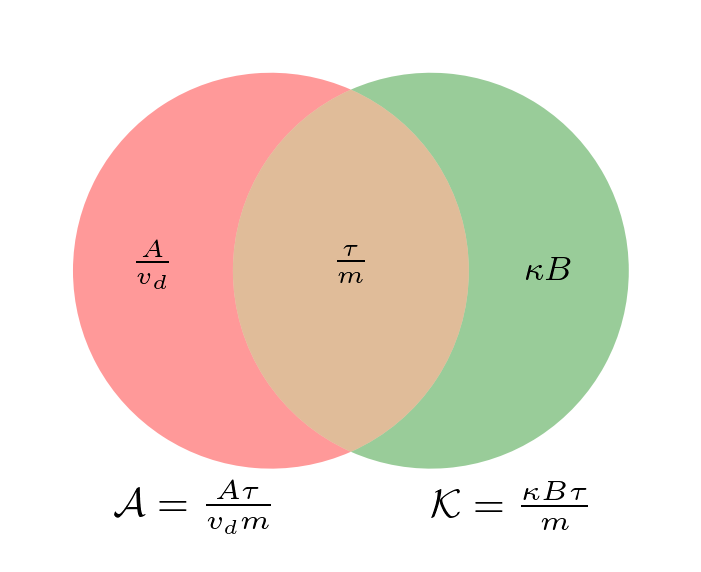
\includegraphics[width=0.49\columnwidth]{./venn_2parameters.png}}
\hfill    
\subfloat[\label{venn_3parameters}]
{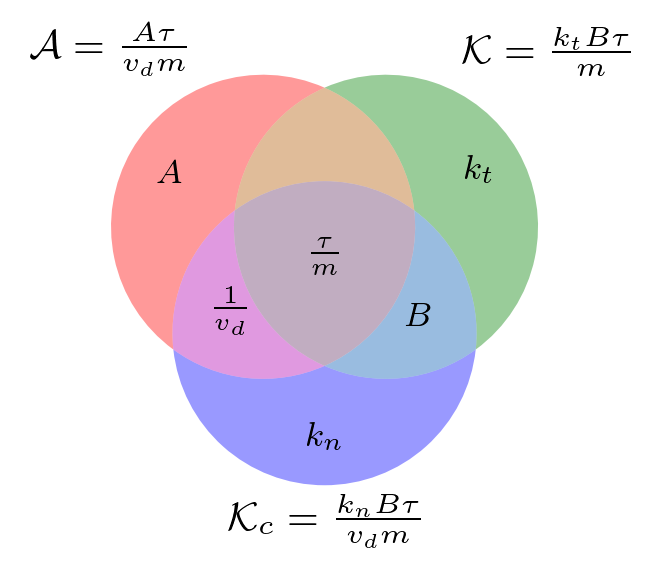
\includegraphics[width=0.49\columnwidth]{./venn_3parameters.png}
}\\
\caption[width=0.47\columnwidth]{Venn diagrams for the \textcolor{blue}{dimensionless} parameters
appearing in the equation of motion (\ref{eqn_motion}) (see 
Appendix~\ref{appendix1} for details). The sets correspond to 
$\mathcal{A}=\{\tau/m,1/v_d,A\}$, $\mathcal{K}=\{\tau/m,B,k_t\}$ and 
$\mathcal{K}_c=\{\tau/m,1/v_d,B,k_n\}$. (a) The Venn diagram representation if no 
body force is introduced in the SFM (only sets $\mathcal{A}$ and $\mathcal{K}$, 
as in Ref.~\cite{dorso_2019}). (b) The Venn diagram representation for the sets 
$\mathcal{A}$, $\mathcal{K}$ and $\mathcal{K}_c$. }
\label{venn_diagram}
\end{figure}

A first inspection of the diagrams in Fig.~\ref{venn_diagram} shows that the 
relaxation time (per unit mass) $\tau/m$ is always a common parameter to all 
sets, regardless of the body force. This means that the ``assertive'' attitude 
of the pedestrian, addressed by the reaction time (see 
Section~\ref{experimental}), applies to all stimuli and the own willings. The 
role of $\tau$ has already been discussed in 
Refs.~\cite{johansson_2009,dorso_2019}.    \\ 

Fig.~\ref{venn_2parameters} represents the situation when $\mathcal{K}_c$ is 
absent. Notice that $A/v_d$ or $k_t B$ may control the collective 
dynamic, in spite of the ``assertive'' attitude. The individual character of 
$v_d$ or $B$ appears somehow ``loosely'' in the crowd dynamic. We mean by 
``loosely'' that any numerical setting of these parameters may be 
counterbalanced by the right setting of $A$ or $k_t$, keeping the 
colletive dynamic (qualitatively) unchanged.  \\

Fig.~\ref{venn_3parameters} provides a picture of the parameters' relations 
after introducing $\mathcal{K}_c$. Surprisingly, $\mathcal{K}_c$ appears as a
wider set (say, a four elements set) than $\mathcal{A}$ or $\mathcal{K}$ (three 
elements' sets). It shares the parameter $v_d$ with $\mathcal{A}$ and the 
parameter $B$ with $\mathcal{K}$. The practical consequence to these (logical)
relations is that $v_d$ or $B$ affect simultaneously two ``control'' parameters 
of the collective dynamics. Conversely, either $v_d$ and $B$ may counterbalance 
$\mathcal{K}_c$ in order to keep the collective dynamic (qualitatively) 
unchanged.  \\

We confirm from these diagrams that no univocal relations can be established 
between the individual parameters and the collective dynamics (in a crowded 
environment). The presence of the body force moves the dynamics to a more 
complex context. We will investigate this context in Section~\ref{results}. \\


\subsection{\label{blocking_clusters} Blocking clusters}

A characteristic feature of pedestrian dynamics is the formation of clusters. Clusters of pedestrians can 
be defined as the set of individuals that for any member of the group (say, $i$) there exists at least
another member belonging to the same group ($j$) in contact with the former. 
Thus, we define a ``granular cluster'' ($C_g$) following the mathematical formula given in Ref.~\cite{strachan1997fragment}

\begin{equation}
C_g:P_i~\epsilon~ C_g \Leftrightarrow \exists~ j~\epsilon~C_g / r_{ij} < (R_i+R_j) \label{ec-cluster}
\end{equation}

where ($P_i$) indicate the \textit{ith} pedestrian and $R_i$ is his (her) radius (shoulder width). That means, $C_g$ is a
set of pedestrians that interact not only with the social force, but also with physical forces (\textit{i.e.} friction force and body force).
A ``blocking cluster'' is defined as the subset of clusterized particles (granular cluster) closest to the door whose first 
and last component particles are in contact with the walls at both sides of the door ~\cite{dorso_2005}.
This clogging structure is responsible for worsening the evacuation performance. 


\section{\label{hypotheses}Working hypotheses and procedures}


\subsection{Working hypotheses}

Our working hypotheses are similar to those mentioned in 
Ref.~\cite{dorso_2019}, 
although the presence of the body force opens inquiries about the proper 
exploration of the parameter space. To be precise

\begin{itemize}
 \item[(a)] The ``faster-is-slower'' (or the ``faster-is-faster'') phenomenon 
occurs when varying the values of $v_d$ (see Section~\ref{bottleneck}). This is 
equivalent to vary simultaneously $\mathcal{A}$ and $\mathcal{K}_c$ by the same 
amount in the (\textcolor{blue}{dimensionless}) parameter space (see Section~\ref{parameters}). We 
may visualize this sampling procedure as moving along a straight line in the 
space $(\mathcal{A},\mathcal{K},\mathcal{K}_c)$. Further variations of 
$k_n$ turns the sample points out of this line, but on the plane of constant
$\mathcal{K}_c$. We will step up $k_n$ by several orders of magnitude in order 
to get the big picture of this surface. 

\item[(b)] We will consider the parameter \textcolor{blue}{set of} Ref.~\cite{helbing_2000} 
as a starting point for exploring the parameter space. The reason for this is 
that a complete set of experimental parameters is still not available (to our 
konwledge). We are aware, though, of the drawbacks \textcolor{blue}{of} this choise, say, the 
unrealistic meanings for the length $B$ and the compressibility $k_n$ (see 
Section~\ref{experimental}). But these are irrelevant in the context of the 
(\textcolor{blue}{dimensionless}) parameter space and the corresponding collective dynamics (see 
Section~\ref{introduction}). 

\item[(c)] We will explore crowd densities allowing body compressions up to 
$0.1\,$m. This corresponds to remarkably high densities, since our own 
(real-life) estimates do not surpass $0.065\,$m (see 
Section~\ref{experimental}). Therefore, the extremely high density 
scenarios (say, above $0.065\,$m) will be considered for the purpose of a 
tendency, but not as a common real-life situation. No casualties due to high 
pressures will be further considered. 

\end{itemize}

We stress the fact that our concern is placed on the collective dynamics of 
crowded environments. We will work on the hypothesis that any ``reasonable'' 
parameter set should reproduce the collective behavior (say, the slowing down 
in the fundamental diagram; see Section~\ref{corridor}). We will not attempt to 
optimize parameters from other objective functions. \\

We will further sustain the hypothesis of soft matter in the context of crowded 
environments. The body compression and the sliding friction parameters are 
supposed to be connected in some way under this hypothesis. However, we will 
not introduce any direct link between $\mathcal{K}$ and $\mathcal{K}_c$. We 
will investigate the interplay between both in Section~\ref{corridor}. 
\\

In order to keep the model as simple as possible, we will only consider 
\textcolor{blue}{isotropic pedestrian interactions}, since \textcolor{blue}{anisotropic
interactions} does not play a relevant role at high densities. \\ 



\subsection{Procedures} 

The SFM was implemented on the LAMMPS simulation software \cite{plimpton}. 
Additional modules for LAMMPS were also written in C++ in order to expand the 
software capabilities. All these were able to run in a high performance 
environment (HPC). \\


The implemented SFM parameters were the same as those in 
Ref.~\cite{helbing_2000} (at the beginning of the exploratory procedure only). 
But the pedestrian's mass and radius were set to the more realistic values of 
$70\,$kg and $0.23\,$m, respectively. The force interactions between 
pedestrians were limited, however, to a cut-off distance of $0.88\,$m for 
attaining a \textit{privacy sphere} \textcolor{blue}{only of the first neighbors}. The desired 
velcity was always set to $1\,$m/s in the corridor situation. Besides, the 
explored values of $v_d$ for the bottleneck scenario ranged from $1\,$m/s to the 
extremely anxious situation of $10\,$m/s. \\


The Eq.~(\ref{eqn_motion}) was numerically integrated by means of the velocity 
Verlet algorithm, with a timestep of $10^{-4}$ seconds. The pedestrians 
positions and velocities were recorded every $0.05\,$sec, but post-processing 
computing was done over samples acquired at least every $2\,$sec., in order to avoid 
data correlations. Those pedestrians leaving the simulations box were 
re-introduced into the box, on the opposite side (periodic boundary 
conditions). We only omitted this mechanism when computing the evacuation time 
for the bottleneck geometry. \\ 


The post-processing computing was assisted by Python functions. The NetworkX 
package was used among others.   \\



\section{\label{results}Results}


\subsection{\label{bottleneck} Bottleneck}


We present in this section the results corresponding to the bottleneck geometry. 
We show the consequences of modifying the body force coefficient $k_n$ on the 
evacuation dynamics. Recall that this coefficient is associated 
to the compression of the human body. \\

Fig.~\ref{vd_vs_te} shows the evacuation time as a function of the pedestrian's 
desired velocity for different values of $k_n$. The evacuation 
time is defined as the time \textcolor{blue}{lapsed} until 80\% of the pedestrians have 
left the room. In this section we will focus on the evacuation time for 
$2\,$m/s$<v_d<10\,$m/s.\\


\begin{figure}[htbp!]
\centering
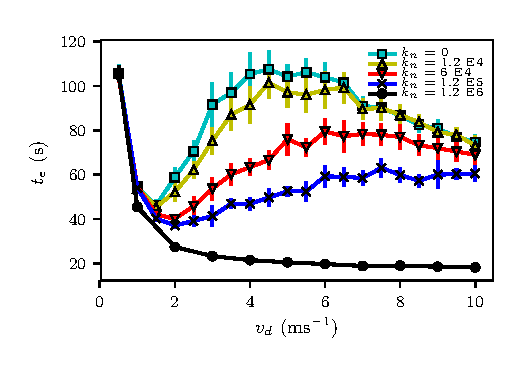
\includegraphics[width=0.7\columnwidth]
{./vd_vs_te_N225.eps}
\caption{\label{vd_vs_te}Mean evacuation time (s) vs. the pedestrian’s desired  
velocity (m/s) for a bottleneck. The room was 20 m x 20 m size. The door was 
0.92 m width (two pedestrians' width). Mean values were computed from 10 evacuation processes. 225 
pedestrians were initially placed in a square lattice with a random initial 
velocity. Each process was finished when 158 pedestrians left the room. The 
different symbols indicate the $k_n$ value corresponding to the body force (see 
the label). The crosses correspond to the Helbing's original SFM parameter, the 
up-triangles correspond to the value measured in 
Ref.~\cite{melvin1988aatd}, squares correspond 
to zero body force and circles correspond to an extreme value of stiffness (one 
order of magnitude higher than the original SFM). The 
 down triangles correspond to an intermediate value between the empirical value 
presented in Ref.~\cite{melvin1988aatd} and the one provided by Helbing in 
Ref.~\cite{helbing_2000} }
\end{figure}

Three behavioral patterns can be distinguished in Fig.~\ref{vd_vs_te}. 
Each pattern can \textcolor{blue}{display} a positive slope, a negative slope
or both. The interval in which the slope is positive means that the 
harder the pedestrians try to get out (higher $v_d$), the 
longer it takes them to evacuate. This is the Faster-is-slower 
(FIS) regime. Conversely, the interval in which the slope is 
negative  corresponds to a Faster-is-Faster (FIF) regime (the 
harder they try, the quicker they leave).\\

Fig.~\ref{vd_vs_te}  shows either FIS or FIF, and a FIS+FIF pattern
for desired velocities $v_d>1.2\,$m/s. The 
evacuation time attains a FIS+FIF pattern for compression coefficients below 
$k=1.2\,$E5. This means that ``soft'' individuals can attain this 
behavioral pattern.  Notice that higher values of $k_n$ allow 
only FIS or FIF patterns. For the highest explored value $k_n=1.2\,$E6, no 
FIS can be seen at all. Besides, the evacuation pattern for $k_n = 0$ and $k_n 
= 2.6\,$E4 are very similar since the body force intensity is of the same order
or less than the social 
force for these stiffness values. \\

Despite the presence of the FIS or FIF pattern, the evacuation time at a 
fixed value of $v_d$ decreases for increasing values of $k_n$ (\textcolor{blue}{within} the examined interval). 
This means that stiffer pedestrians evacuate faster than soft pedestrians. 
To further investigate this 
phenomenon, we computed the mean velocity of the whole crowd as a function of the 
stiffness $k_n$. Fig.~\ref{kn_vs_vx_bottleneck} shows the actual mean velocity in the 
$x-$direction as a function of the stiffness $k_n$ for three different desired 
velocities. In all cases, the velocity increases with the stiffness. The most significative 
increment of velocity is in the interval \textcolor{blue}{$k_n>\,10^{4}$}. \\


\begin{figure}[!htbp]
\centering
    \subfloat[]{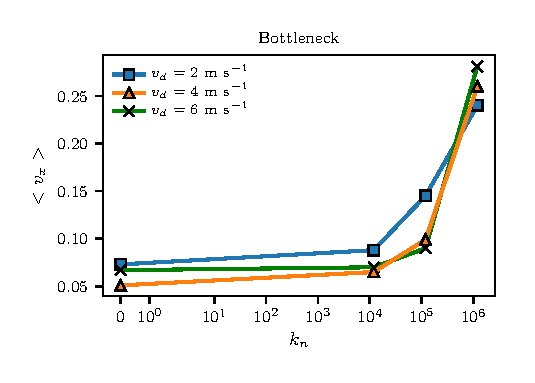
\includegraphics[width=0.7\columnwidth]{./kn_vs_vx_bottleneck.eps}}\\
\caption[width=0.47\columnwidth]{Mean velocity in the $x-$direction as a function 
of the stiffness level $k_n$ for different desired velocities (see label). The 
data corresponds to a bottleneck with periodic boundary conditions (re-injecting 
pedestrians). The average was taken every five seconds once the crowd reaches the 
stationary state ($t=20\,$s) until the end of the simulation ($t=1000\,$s). 
Color online only. }
\label{kn_vs_vx_bottleneck}
\end{figure}


The existence of the FIF phenomenon for only ``stiff'' individuals opens many questions 
on the microscopic dynamics of pedestrians. We may presume that contacts 
between pedestrians are quite different for soft individuals than for stiff 
individuals. Thus, we proceed to study the dynamics of contacting pedestrians, regardless of the overlap 
effects. We will assimilate the pedestrians as nodes and the whole crowd as a 
network. We will link any two individuals whenever they get in physical 
contact (\textit{i.e.} $r_{ij} \leq R_{ij}$).\\

Fig.~\ref{degree_vd} shows the mean degree of the contact network as a function  
of the desired velocity. The degree of a node is defined as the number of links 
that \textcolor{blue}{connects} this node to any other node. This means, the number of pedestrians 
that are in physical contact with a given pedestrian. The mean degree is the 
average of the degree over all the nodes (pedestrians) and over the whole 
sampled interval. We computed mean values only after the system reached the stationary 
state, that is, after a well-formed bulk has been established.\\

Notice that the mean degree increases as $v_d$ increases, as expected. This expresses the fact that
higher $v_d$ values accomplish higher densities, \textcolor{blue}{forcing} individuals to touch each 
other. For a given $v_d$, the mean degree reduces as the $k_n$ 
value increases. A noticeable decrease in the mean degree can be seen for the 
highest explored value of $k_n$. This \textcolor{blue}{was not expected and} opens the question on how would
this affect the sliding friction among pedestrians.\\

A more detailed insight into the contact dynamics can be acquired from 
Fig.~\ref{overlap_vd}. The overlap between individuals is shown as a function of 
$v_d$. Recall from Section \ref{sfm} that the overlap is defined as 
$R_{ij}-r_{ij}$ where $R_{ij}$, is the sum of radius of particle $i$ and 
particle $j$ and $r_{ij}$  is the distance between both particles. Except for 
very low desired velocities (say, $v_d<2\,$m/s), we can see that the mean 
overlap is an increasing function of $v_d$ (withing the studied
range of $v_d$ and $k_n$).\\


\begin{figure}[!htbp]
\centering
    \subfloat[]{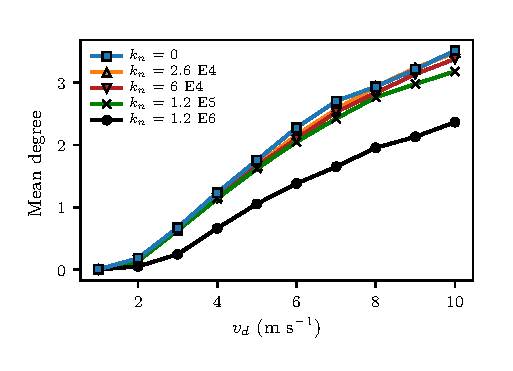
\includegraphics[width=0.49\columnwidth]{./degree_vs_vd_multi_kn.eps}\label{degree_vd}}\ 
    \subfloat[]{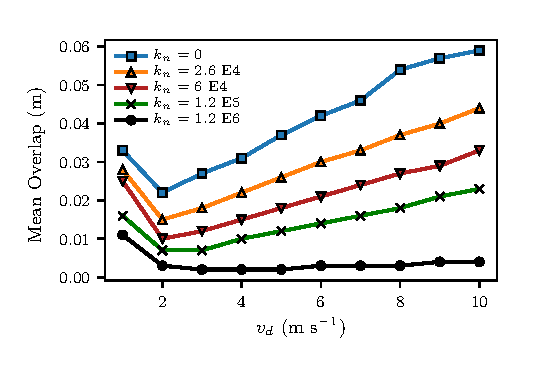
\includegraphics[width=0.49\columnwidth]{./overlap_vs_vd_multi_kn.eps}\label{overlap_vd}}\\
\caption[width=0.47\columnwidth]{(a) Mean degree as a function of the pedestrian’s desired velocity (m/s). (b) Mean overlap as a function of the pedestrians desired velocity. Each symbol indicates the $k_n$ value corresponding to the body force (see the labels). The data corresponds to a bottleneck with periodic boundary conditions (re-injecting pedestrians). The average was taken over time and the pedestrians in the bottleneck. The sampling was done every five seconds once the crowd reached the stationary state (say, $t=20\,$s) until the end of the simulation ($t=1000\,$s). Color online only.}
\label{degree_overlap_vd}
\end{figure}

The regime for $v_d<2\,$m/s is qualitatively different from the clogged regime since most of the 
pedestrians are not touching each other (as was already observed in Ref~\cite{dorso_2005,dorso_2011}). The only pedestrians who touch each 
other are the ones who are being re-injected on the opposite side of the room.
\textcolor{blue}{These collide with the bulk}, providing some kind of overlap during very short time. We will
not analize this regime.\\

Besides, for a given $v_d>2\,$m/s, the overlap increases as the $k_n$ value decreases. 
This can be explained by considering the bulk at a (quasi) equilibrium situation. 
The social and compression forces counterbalance the desired force. Thus, for any fixed $v_d$,
the product $k_n \times (R_{ij}-r_{ij})$ remains (almost) fixed. Any decrease in $k_n$
allows a more significant intrusion. This (partially) supports the argument that
the sliding friction should weaken for stiffer pedestrians (say increasing
$k_n$ values). \\  


The sliding friction reduction appears as the first feature for enhancing
the overall evacuation performance. Either reducing the mean overlap and the mean degree
tend to diminish the mean sliding 
friction within the crowd. 
Notice, however, that switching from a FIS regime (positive slope) to a  FIF 
regime (negative slope) in Fig.~\ref{vd_vs_te} appears as a more complex 
phenomenon. We will focus on this issue in an upcoming investigation.\\

The body force 
has a notorious impact in the number of pedestrians touching each other (say, 
the degree). This is clearly depicted in Fig.~\ref{network_bottleneck} where 
four different configurations of the evacuation dynamics are shown. The 
configurations represent 225 pedestrians trying to escape through a door (see 
caption for details). The colors correspond to the degree of each node 
(pedestrian), and the lines between pedestrians represent the contacts among 
them.\\



\begin{figure}[!htbp]
\centering
    \subfloat[]{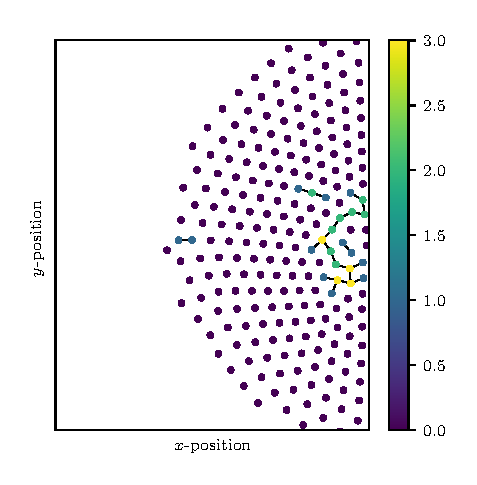
\includegraphics[width=0.49\columnwidth]{./network_vd2_kn0.eps}\label{network_vd2_kn0}}\ 
    \subfloat[]{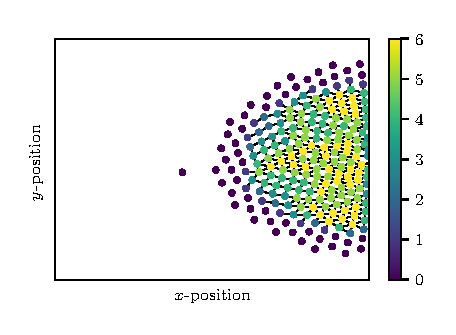
\includegraphics[width=0.49\columnwidth]{./network_vd10_kn0.eps}\label{network_vd10_kn0}}\\
        \subfloat[]{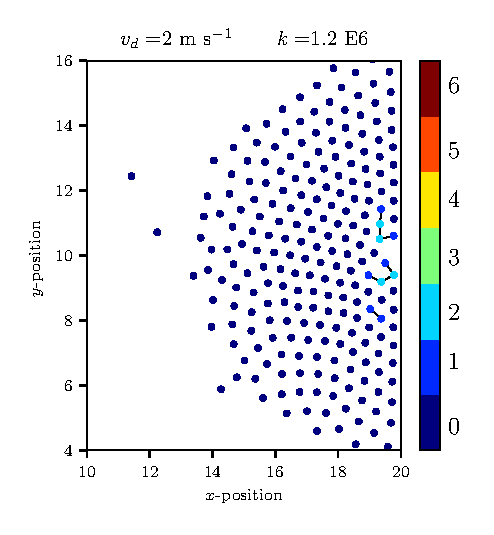
\includegraphics[width=0.49\columnwidth]{./network_vd2_kn1200000.eps}\label{network_vd2_kn1200000}}\ 
    \subfloat[]{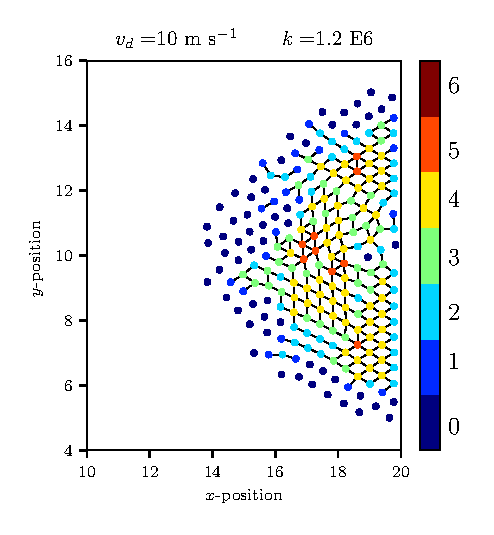
\includegraphics[width=0.49\columnwidth]{./network_vd10_kn1200000.eps}\label{network_vd10_kn1200000}}\\
\caption[width=0.47\columnwidth]{Snapshots of the contact networks of a 225 pedestrian evacuation through a bottleneck. The door is placed at $(x,y)=(20,10)\,$m, the width of the door is 0.92$\,$m (equivalent to 2 pedestrian\textsc{\char13}s diameter). The lines that connect the nodes (pedestrians) represent the contact between them. The color represents the degree (the number of pedestrians with which it is connected). (a) and (b) correspond to a simulation without body force with $v_d=$2 and $v_d=$10 respectively. (c) and (d) correspond to simulations with $k_n=1.2\,$E6 with $v_d=$2 and $v_d=$10 respectively. Color online only.}
\label{network_bottleneck}
\end{figure}



The four configurations corresponds to two different $v_d$ and two different $k_n$ values (say, the  minimum and maximum explored values). Fig.~\ref{network_vd2_kn0} and Fig.~\ref{network_vd10_kn0} show snapshots for $k_n=0$, at the desired velocities of 2$\,$m/s and 10$\,$m/s, respectively.    Fig.~\ref{network_vd2_kn1200000} and Fig.~\ref{network_vd10_kn1200000} show similar situations, but for  $k_n=1.2\,$E6. As expected, increasing the desired velocity compresses the crowd towards the exit. \\

The four snapshots in Fig.~\ref{network_bottleneck} confirm (visually) the fact that more rigid pedestrians \textcolor{blue}{ease} the crowded environment, widening the occupied region. At $v_d=10\,$m/s (the maximum explored velocity), it can hardly be found pedestrians with degree 6 when $k_n=1.2\,$E6, while a lot of them are present for $k_n$=0.\\

The clusterization of the pedestrians has a significant impact on the blocking clusters (the group of pedestrians that clog the exit).  Fig.~\ref{pbc_vs_vd_multi_kn} shows the blocking cluster probability as a function of the desired velocity for different $k_n$ values (see caption for details). The blocking clusters become more probable for high desired velocity, since the clogged area gets more compact as $v_d$ increases (for any fixed value of $k_n$). But, the most remarkable fact in Fig.~\ref{pbc_vs_vd_multi_kn} is that increasing the body stiffness reduces the blocking cluster probability for any fixed value of $v_d$. Recall from Ref.~\cite{dorso_2005} that the evacuation time is controlled by the blocking. Thus, increasing the body stiffness affects the presence of the blocking clusters, and consequently improves the evacuation time. This raises as a second feature for enhancing the overall evacuation performance. \\

\begin{figure}[htbp!]
\centering
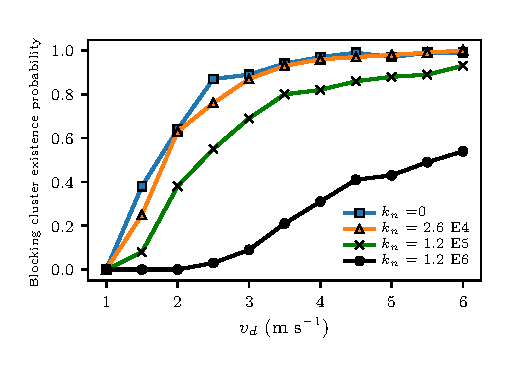
\includegraphics[width=0.7\columnwidth]
{./pbc_vs_vd_multi_kn.eps}
\caption{\label{pbc_vs_vd_multi_kn} Blocking cluster probability as a function of $v_d$ for different stiffness levels (see label). The probability is calculated as the amount of time a blocking cluster is present divided by the overall simulation time. The situation corresponds to a bottleneck with 225 pedestrians under periodic boundary conditions (re-injection of pedestrians once they left the room). The sampled interval was set to $t_f =$ 1000$\,$s. Color online only. }
\end{figure}

We may summarize this Section as follows. We explored the parameter space along $v_d$ and $k_n$ for the bottleneck situation. This is similar to explore the \textcolor{blue}{dimensionless} plane $(\mathcal{A},\mathcal{K}_c)$. Soft pedestrians attain a FIS or FIS+FIF evacuation pattern but, stiff pedestrians (for any fixed $\mathcal{A}$ value within the explored range) exhibit a single FIF pattern. Stiffness affects either the presence of the blocking clusters and the pedestrians overlap. The less they overlap, the less intense becomes the sliding friction among them. Additionally, the fewer the blocking clusters the easier they get out. \\



\subsection{\label{corridor} Corridor}

We present in this section the results corresponding to the corridor geometry. 
We show the effects of modifying the body force coefficient $k_n$ on the 
collective dynamics. We will keep $v_d$ (or $\mathcal{A}$) 
fixed along this Section. \\

We first computed the contact network in the same way 
as in the bottleneck geometry. Fig.~\ref{degree_dens} shows the 
mean degree as a function of the global density for different $k_n$ values (see 
caption for details). The mean degree vanishes at very low 
densities because the pedestrians do not touch each other. When the density 
surpasses 4.5, a few pedestrians start to touch each other, 
raising the mean degree. As the density continuous increasing, 
the mean degree approaches the asymptotic value 
of six. Degree six corresponds to the maximum packing density for identical 
hard circles.\\


\begin{figure}[!htbp]
\centering
    
\subfloat[]{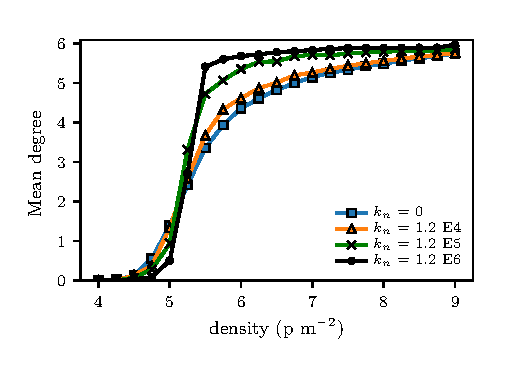
\includegraphics[width=0.49\columnwidth]
{./degree_vs_dens_multi_kn.eps}\label{degree_dens}}\ 
\subfloat[]{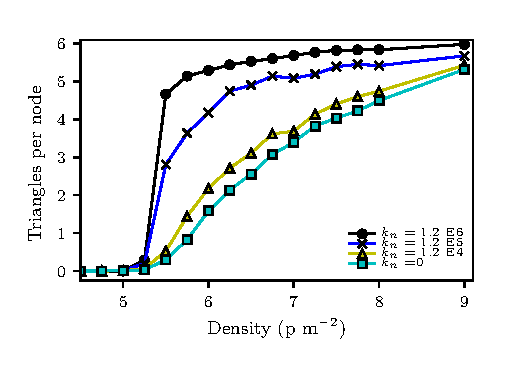
\includegraphics[width=0.49\columnwidth]
{./triangles.eps}\label{triangles}}\\
% \subfloat[]{\includegraphics[width=0.49\columnwidth]
%{./overlap_vs_dens_multi_kn.eps}\label{overlap_dens}}\\
\caption[width=0.47\columnwidth]{(a) Mean degree as a function 
of the global density for different $k_n$ values. (b)  Triangles per node as a 
function of the global density. The global density is the total number of 
pedestrians per unit area. The mean values are averages over all the pedestrians 
and over time once the system reached the stationary state. The measurements 
correspond to a corridor of 28~m $\times$ 22~m with periodic boundary conditions 
and $v_d=1$. Color online only.}
\label{network_corridor}
\end{figure}


It is worth noting from Fig.~\ref{degree_dens} that ``stiff''
pedestrians exhibit a sharper transition to the maximum packing density than 
the ``soft'' pedestrians. We further checked this phenomenon by counting the 
number of loops of three nodes (say, the triangles) present in the network. 
This magnitude was reported to be a sensitive magnitude for characterizing the 
jamming transition in a compressed granular packing (see 
Ref.~\cite{pugnaloni_2013} for details).  As can be seen in 
Fig.~\ref{triangles}, the ``stiff'' pedestrians share more triangles 
than the ``soft'' ones.   \\

In order to get a better insight on how the pedestrians contact to each other, 
we present in Fig.~\ref{network_corridor} two snapshots of the corridor at the 
stationary situation. Fig.~\ref{network_d6_kn0} corresponds to 
$k_n=0$, while Fig.~\ref{network_d6_knE5} corresponds to $k_n=1.2$~E5. The 
former shows a somewhat disordered network, while the latter exhibits an almost 
completely ordered lattice. The missing triangles in Fig.~\ref{network_d6_kn0} 
are replaced by other polygons of more than three edges.    \\


\begin{figure}[!htbp]
\centering
    \subfloat[]{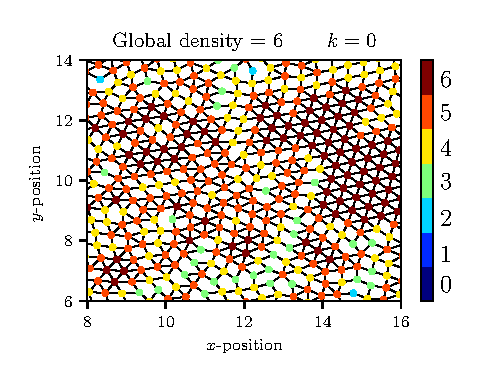
\includegraphics[width=0.49\columnwidth]{./network_d6_kn0.eps}\label{network_d6_kn0}}\ 
    \subfloat[]{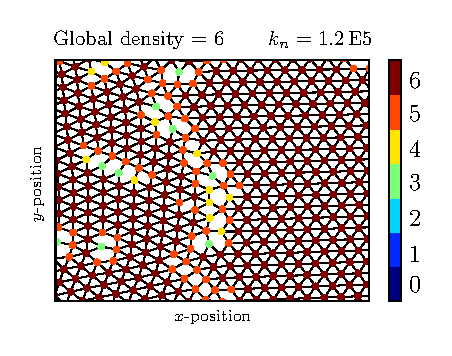
\includegraphics[width=0.49\columnwidth]{./network_d6_knE5.eps}\label{network_d6_knE5}}\\
\caption[width=0.47\columnwidth]{Contact network of the pedestrians along the corridor at time $t=50\,$s. The global density was $\rho=6$.  The lines that connect the nodes (pedestrians) represent the contact between them. The colors stand for the degree of the node (the number of pedestrians that are in contact with him/her). The corridor was 28~m $\times$ 22~m with periodic boundary conditions and $v_d=1$. (a) corresponds to a simulation without body force and (b) corresponds to a simulation with $k_n=1.2$~E5. The friction coefficient and the other SFM parameters are the same as in Section \ref{bottleneck}. Color online only.}
\label{network_corridor}
\end{figure}

We find these topological magnitudes useful for comparing the 
corridor geometry with respect to the bottleneck geometry. A re-examination of 
Fig.~\ref{degree_dens} (corridor) and Fig.~\ref{degree_vd} (bottleneck) reveal 
that the pedestrian stiffness $k_n$ affects differently the way they contact 
each other. The mean degree increases for ``stiff'' pedestrians moving along 
the corridor (at densities above $5\,$p/m$^2$). Conversely, the mean degree 
increases for ``soft'' pedestrians in the bottleneck situation.\\  

Fig.~\ref{network_bottleneck} and 
Fig.~\ref{network_corridor} illustrate the connectivity differences between 
the bottleneck and the corridor situation. The bulk in 
Fig.~\ref{network_bottleneck} appears more heavily connected among ``soft'' 
pedestrians than among ``stiff'' pedestrians (see both snapshots at $v_d=10$). 
The opposite occurs in Fig.~\ref{network_corridor}. This discrepancy seems to 
be related to the boundary conditions, since the same SFM parameters were 
applied on both situations. We may speculate that this phenomenon occurs 
because, in the corridor, the lateral walls act like a containment barrier that 
forces the ``stiff'' pedestrian to increase his (her) contacts. On the contrary, 
no real containment walls exist in the bottleneck situation (regardless the side 
walls). \\



We can test our hypothesis by computing the mean overlap. 
Fig.~\ref{overlap_dens} shows this magnitude for the corridor situation. Notice 
that ``soft'' pedestrians attain a more intruding overlap than the ``stiff'' 
ones, as expected. This is in agreement with Fig.~\ref{overlap_vd} for the 
bottleneck situation (at a fixed value of $v_d$). The curves in 
Fig.~\ref{overlap_vd}, however, do not meet each other as in  
Fig.~\ref{overlap_dens}. The curve meeting attains for space limitations in 
the corridor, since overlapping occurs (almost) independently of the value of
$k_n$. This is clearly not the case in the bottleneck situation. \\



\begin{figure}[htbp!]
\centering
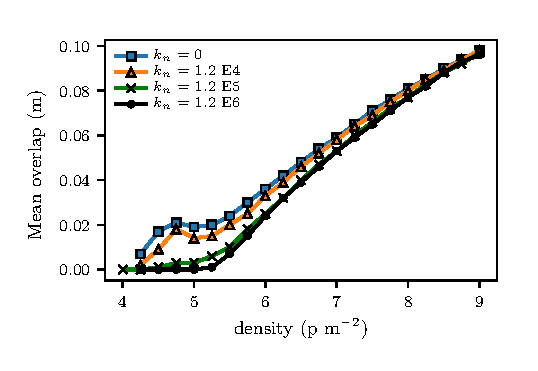
\includegraphics[width=0.7\columnwidth]
{./overlap_vs_dens_multi_kn.eps}
\caption{\label{overlap_dens} Mean overlap as a function of the 
global density. The global density is the total number of pedestrians per unit 
area. The mean values are averages over all the pedestrians and over time once 
the system reached the stationary state. Both measurements correspond to 
the corridor geometry with desired velocity $v_d=1$. Color 
online only. }
\end{figure}


The above results correspond to a milestone in the 
investigation. The connectivity differences between the bottleneck geometry 
and the corridor geometry were not expected and opens two major questions: how 
does the body stiffness interact with the walls, and consequently, how does 
this affect the flux across the corridor.\\ 

We start by computing the mean velocity across the corridor.  
Fig.~\ref{kn_vs_vx_corridor} shows the mean velocity 
$\langle v_x\rangle$ (parallel to the corridor) as a function 
of the stiffness for different global density levels. This 
plot shows a flat pattern for $k_n<10^4$ and a slowing down above this 
threshold. Notice from Fig.~\ref{kn_vs_vx_bottleneck} that this is opposed
to what happens in the bottleneck geometry. \\


\begin{figure}[htbp!]
\centering
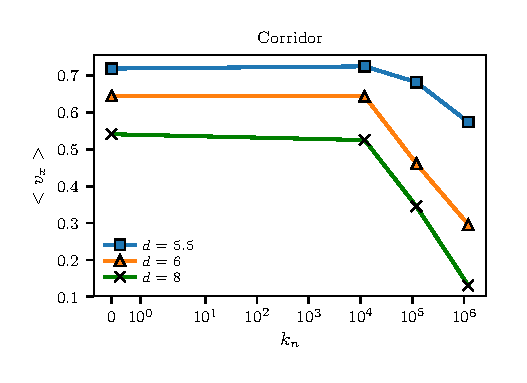
\includegraphics[width=0.7\columnwidth]{./kn_vs_vx_corridor.eps}
\caption{\label{kn_vs_vx_corridor} Mean velocity in the longitudinal coordinate $(v_x)$
 as a function of the stiffness $k_n$ for three different global densities (see label in the plot). 
 The measurements correspond to a corridor of 28~m $\times$ 22~m with periodic boundary conditions and $v_d=1$.
 The average was taken along the corridor and along the simulated time. Color online only.      }
\end{figure}

The $\langle v_x\rangle$ values in Fig.~\ref{kn_vs_vx_corridor} 
were computed at densities $\rho\geq 5.5$. According to 
Fig.~\ref{overlap_dens}, these densities attain relevant overlaps. Furthermore, 
stiffness values $k_n\geq 10^4$ move the system to a more heavily connected 
stage, and thus, pedestrians have no choice but to walk at 
(almost) the same speed as his (her) neighbors. This 
behavior may be envisaged as the passage from a released 
walking movement to a tigh movement as the stiffness increases. A more 
physical picture would assimilate te former as a ``fluid-like 
state'' and the latter as a ``solid-like state''. When the stiffness is 
very high (say $k_n=$1.2~E6), all the pedestrians 
are expected to walk at a common velocity. The 
pedestrians that walk in physical contact with the wall are the ones who 
determine the velocity of the whole crowd, as discussed 
below.\\

Fig.~\ref{vx_profile} shows the velocity profile ($\langle v_x \rangle$ vs. the transversal coordinate $y$) for different $k_n$ values. For $k_n=0$, we can see a parabolic-like velocity profile that resembles the Poiseuille flow (similar to Newtonian and incompressible fluids in a laminar regime). This behavior was also observed in empirical measurements of crowd dynamics reported in Ref.~\cite{zhang2013empirical}. But as $k_n$ increases the velocity profile flattens until becoming (almost) uniform (see Fig.~\ref{vx_profile} for $k_n=1.2\,$E6). In this scenario, $v_x$ attains a much lower level than in the case of soft pedestrians ($k_n=$0).\\

The crowd behaves like a solid for very stiff pedestrians. This means that the crowd can not be easily ``deformed''. In this context, deformation means that parts of the crowd may be released to move faster than other parts of the crowd. \\

The strain rate is the tensor that expresses how the relative velocity of a medium changes when one moves away from one position to another. We consider the following discrete definition of the strain rate:

\begin{equation}
S = \frac{\langle v_x(\mathrm{center})\rangle - \langle v_x(\mathrm{boundary})\rangle }{\left | y(\mathrm{center}) - y(\mathrm{boundary}) \right |} 
\end{equation}


\begin{figure}[!htbp]
\centering
    \subfloat[]{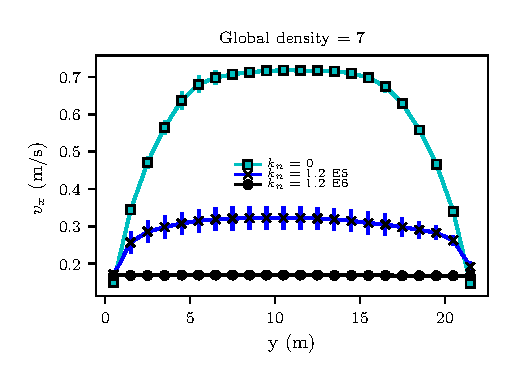
\includegraphics[width=0.49\columnwidth]{./vx_profile.eps}\label{vx_profile}}\ 
    \subfloat[]{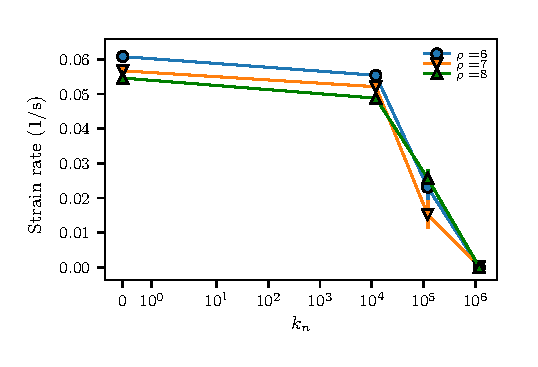
\includegraphics[width=0.49\columnwidth]{./strain_rate_vs_kn.eps}\label{strain_rate_vs_kn}}\\
\caption[width=0.47\columnwidth]{(a) Mean velocity in the $x$ coordinate as a function of the transversal coordinate $y$ for three different stiffness values $k_n$ (see the label). (b) Strain rate as a function of the stiffness level $k_n$ for three different global density values (see label). Data correspond to a corridor of 28$\,$m $\times$ 22$\,$m with periodic boundary conditions and $v_d=1$. The global density was $\rho=7 p\,$m$^{-2}$. Color online only. }
\label{profile_strain}
\end{figure}

Where $\langle \cdot \rangle$ means the average taken over time. This definition compares the velocity of the pedestrians close to the wall (boundary) with respect to the velocity of the pedestrians at the center of the corridor (center). Thus, $S$ vanishes (no deformation) as the stiffness level increases. This phenomenon is shown in Fig.~\ref{strain_rate_vs_kn} where we can see that the strain rate drops for high values of $k_n$. \\


We conclude this Section by stressing that stiffer pedestrians attain opposite results in corridors with respect to bottlenecks. The walls in the corridors play a critical role that prevents pedestrians from detaching from each other. This effect has can be observed as an increment in the connectivity of the contact network and the flattening of the velocity profile (thus reducing the strain rate). Very high enough stiffness values stuck the pedestrians leading to a ``solidification'' of the crowd. All the pedestrians walk at almost the same velocity at this stage. The pedestrians that are in contact with the walls are the ones that determine the velocity of the whole crowd. We already analyzed this situation in Ref~\cite{dorso_2019}. \\

\subsection{Dimensionless numbers and comparison with empirical data}


IThe final stage of our investigation deals with the plausible values of the dimensionless numbers $\mathcal{K}_c$ and $\mathcal{K}$, in comparison to the empirical measurements. We vary the body force coefficient ($k_n$) and the friction coefficient ($k_t$) to explore different values of $\mathcal{K}_c$ and $\mathcal{K}$, respectively.\\

We consider the empirical measurements from Ref.~\cite{helbing_2007} corresponding to the fundamental diagram obtained at the entrance of the Jamaraat bridge (see the inset in Fig.~\ref{flow_density_no_body_force}). Our aim is to reproduce the qualitative behavior of these measurements.\\

Figs. \ref{flow_density} show the pedestrian flow as a function of the global density (fundamental diagram). Fig.~\ref{flow_density_no_body_force} corresponds to $\mathcal{K}_c=$ 0 (this is \textit{i.e.} $k_n=0$) while Fig.~\ref{flow_density_body_force} corresponds to $\mathcal{K}_c=$68 corresponding to the original SFM with $k_n=1.2\,$E5. Each curve represents different friction values (see the caption for details).\\

According to the empirical measurements at Jamaraat, the flow slows down for high enough densities due to jamming. Notice that the original SFM (corresponding to $\mathcal{K}=$137) does not produce the expected slowing down for null body force ($\mathcal{K}_c=$0). However, when the body force is present (the original SFM) an ``U'' shape behavior occcurs for densities above 5 p$^{-2}$.\\

The increase in $\mathcal{K}$ to $\mathcal{K} = $ 685 (five times the original SFM value) slows down  the flux for densities above 5 p m$^{-2}$, regardless of the presence of the body force. Including the body force, however, produces a subtle increment in the flow for densities higher than 7 p m$^{-2}$ (see orange curve from Fig.~\ref{flow_density_no_body_force}). \\

A further increment of $\mathcal{K}$ to $\mathcal{K}=$137 (ten times the original SFM value) attains a plateau ($\rho>5$ p m$^{-2}$) before vanishing at very high densities. This occurs on either $\mathcal{K}_c=$ 0 and $\mathcal{K}_c = $ 68.\\

%It is worth mentioning that the SFM contemplates the possibility of overlapping between pedestrians (unlike the models stated in Refs.~\cite{kabalan_2017,jebrane_2019}). Despite this hard-to-interpret feature, the SFM can reproduce empirical behaviors of collective pedestrian dynamics.\\

These results suggest that although increasing $\mathcal{K}_c$ slows down the flux, it is still necessary to increase $\mathcal{K}$ (by increasing the friction coefficient $k_t$) to avoid an ``U'' shape behavior for extremely high densities. It is still a challenge to find the optimal dimensionless numbers  $(\mathcal{A},\mathcal{K},\mathcal{K}_c)$ for the fundamental diagram. Our inspection into the parameter set is a first approach to narrow down the search.\\

\begin{comment}
Fig. \ref{flow_density} shows the flow as a function of the global density (fundamental diagram). \ref{flow_density_no_body_force} corresponds to zero body force (\textit{i.e.} $k_n=0$), Fig.~\ref{flow_density_body_force} corresponds to a body force with $k_n=1.2\,$E5. Each curve correspond to a different friction value (see the caption).\\

According to most of the empirical measurements, the flow decreases for high enough values of density because the crowd becomes jammed. Notice that the original friction does not produce a reduction of the flow when there is zero body force but when the body force is included (with the original SFM value), the flow reduces from  5 p m$^{-2}$ to 7 p m$^{-2}$ and increases for higher values of density. When the friction is five times the original value, the flow reduces for densities higher than 5 p m$^{-2}$ in both cases (with body force and without body force). The main qualitative difference is that including the body force produces a subtle increment in the flow for densities higher than 7 p m$^{-2}$. When the friction is increased by a factor of ten, the flow reduces or remains constant when the density is higher than 5 p m$^{-2}$ for both cases (with body force and without body force). This result suggests that even including the body force, the original SFM requires an increment of the friction in order to reproduce the flow reduction reported in empirical measurements.\\
\end{comment}

\begin{figure}[!htbp]
\centering
    \subfloat[]{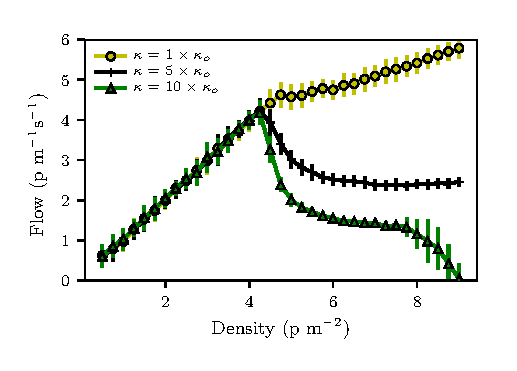
\includegraphics[width=0.49\columnwidth]{./flow-density_multifric_nobodyforce.eps}\label{flow_density_no_body_force}}\ 
    \subfloat[]{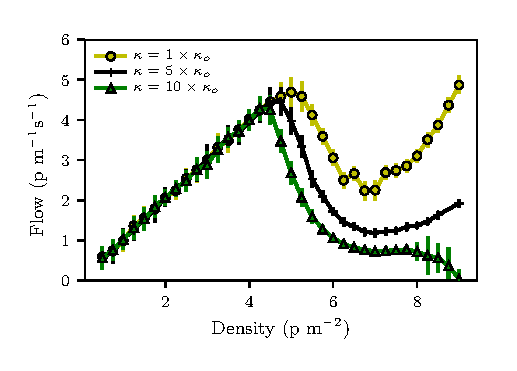
\includegraphics[width=0.49\columnwidth]{./flow-density_multifric_bodyforce.eps}\label{flow_density_body_force}}\\
\caption[width=0.47\columnwidth]{Flow vs. global density. The flow is calculated in a circular area of $R=1\,$m at the center of the corridor. The circular markers correspond to the original friction of the SFM, the "+" symbol corresponds to the friction increased by a factor of five and the triangles correspond to the friction increased by a factor of ten. The desired velocity was $v_d=1$ in all the cases. (a) corresponds to simulations without body force ($\mathcal{K}_c =$0) and (b) corresponds to a body force with the original value of the body stiffness ($\mathcal{K}_c =$68). Color online only.}
\label{flow_density}
\end{figure}



\section{\label{conclusions}Conclusions}


We explored the effect on the pedestrians dynamics of the (sometimes neglected) body force in the framework of the SFM. We showed that the stiffness coefficient ($k_n$) has a significant impact on the evacuation dynamics (bottleneck) and also in the dynamics of pedestrians walking along a straight corridor.\\

In the bottleneck geometry, the evacuation time diminishes (pedestrians move faster) as pedestrians become stiffer along the explored desired velocities. This phenomenon occurs because stiffer pedestrians reduce the overlapping and hence the sliding friction intensity. This scenario releases more easily the pedestrians and reduces the probability of producing a cluster of pedestrians blocking the exit (blocking cluster). This leads to a more efficient evacuation dynamics. \\

The opposite behavior is obtained in the corridor geometry with respect to the bottleneck geometry. The major difference is that pedestrians are limited to the available space between walls in the corridor geometry.  Walls are not relevant in the bottleneck geometry. Thus, the overlap between pedestrians is controlled by the available space. But, stiffer pedestrians are more likely to get stuck. The whole crowd can be compared to a granular material. Granular materials can be disordered (amorphous) or ordered depending on how particles link to each other. In the present context, at low stiffness levels, the crowd appears disordered attaining a parabolic velocity profile.
If the stiffness level is high, the whole crowd appears ordered into a lattice (like a crystalline solid) with a uniform velocity profile that depends on the friction interaction with the walls.\\

Our efforts to ``tune'' the original SFM to empirical data (say, the fundamental diagram) moved us to explore the dimensionless parameter space.  We found that the qualitative behavior of empirical  data can be accomplished if the parameters are close to $\mathcal{K}_c < 68$, $\mathcal{K} = 685$ and $\mathcal{A}=14$. Nevertheless, this is a first attempt to arrive at suitable parameters, although we do not claim these to be optimal. We encourage further research to find dimensionless numbers that may better fit experimental data.\\


\section*{Acknowledgments}
This work was supported by the National Scientific and Technical 
Research Council (spanish: Consejo Nacional de Investigaciones Cient\'\i ficas 
y T\'ecnicas - CONICET, Argentina) grant Programaci\'on Cient\'\i fica 2018 (UBACYT) Number 20020170100628BA.\\

The authors want to thanks the degree students Josefina Catoni and Ayelen Santos for providing data acquired at 
the subway in Buenos Aires, Argentina. 

\appendix

\section{\label{appendix1}Reduced-in-units equation of motion}

The SFM description in section~\ref{sfm} introduces seven parameters ($m$, 
$\tau$, $v_d$, $B$, $A$, $k_t$ and $k_n$) attaining for the ``individual'' 
behavior of each pedestrian. The collective dynamic, however, requires a 
smaller set of parameters. In order to identify this smaller set, we introduce 
the following \textcolor{blue}{dimensionless} magnitudes\\

\begin{equation}
 \left\{\begin{array}{lcl}
         t' & = & t/\tau \\
         r' & = & r/B \\
         v' & = & v/v_d \\
        \end{array}\right.
\end{equation}

The equation of motion (\ref{eqn_motion}) can be \textcolor{blue}{rewritten} in terms of these 
(\textcolor{blue}{dimensionless}) magnitudes, while only three (reduced) parameters are needed.\\


\begin{equation}
 \displaystyle\frac{d\mathbf{v}'}{dt'}=
 \hat{\mathbf{e}}_d-\mathbf{v}'+\mathcal{A}\,e^{R'-r'}\,
 \hat{\mathbf{n}}+g(R'-r')\,\bigg[\mathcal{K}\,(\Delta\mathbf{v}'\cdot
 \hat{\mathbf{t}})\,\hat{\mathbf{t}}+\mathcal{K}_c\,\hat{\mathbf{n}}\bigg]
\end{equation}



\noindent where the smaller set ($\mathcal{A}$,$\mathcal{K}$,$\mathcal{K}_c$) 
means\\

\begin{equation}
 \mathcal{A}=\displaystyle\frac{A\,\tau}{m\,v_d}\ \ \ \ , \ \ \ \ 
 \mathcal{K}=\displaystyle\frac{k_t\,B\,\tau}{m}\ \ \ \ , \ \ \ \
 \mathcal{K}_c=\displaystyle\frac{k_n\,B\,\tau}{m\,v_d}
\end{equation}

Notice that the SFM will arrive to similar collective dynamics whenever the 
reduced set ($\mathcal{A}$,$\mathcal{K}$,$\mathcal{K}_c$) remains unchanged 
(although some ``individual'' parameters are allowed to change). For a deep 
explanation on the meaning  of the set 
($\mathcal{A}$,$\mathcal{K}$,$\mathcal{K}_c$) see section~\ref{parameters}. \\




%/////////////////////////////////////////////////
%\begin{thebibliography}{10}
%\expandafter\ifx\csname url\endcsname\relax
%  \def\url#1{\texttt{#1}}\fi
%\expandafter\ifx\csname urlprefix\endcsname\relax\def\urlprefix{URL }\fi
%\expandafter\ifx\csname href\endcsname\relax
%  \def\href#1#2{#2} \def\path#1{#1}\fi

%\bibitem{helbing3}
%Helbing, D., Johansson, A., and Al-Abideen, H. Z., 2007. ``Dynamics of crowd 
%disasters: An empirical study." Physical review E 75 (4), 046109.
%{\path{https://doi.org/10.1103/PhysRevE.75.046109}}

%\end{thebibliography}

\bibliographystyle{unsrt}
\bibliography{paper}% Produces the bibliography via BibTeX.

\end{document}
\endinput

